\documentclass[fleqn,12pt]{article}
\usepackage{mathsx,bigpage,tikz}
\usepackage{questions}

\usepackage{scalalistings}
\def\Programming{\textbf{[Programming]}}
\def\scalacolour{\color{blue}}

%% \questionsonly
%% \questionsandanswers
%\answersonly
%\nontuteanswersonly

\title{Concurrent Programming: Exercise Sheet 2}
\author{Gavin Lowe}

\sloppy

\begin{document}
\maketitle

% Deadline (for Department classes): Friday Week 4.

You should complete all questions marked \Programming\ at a computer.

Questions marked $\dagger$ will not normally be discussed in class.  Model
answers are included below.  You should attempt these questions and mark them
yourself; ask your tutor if they would like them to be handed in.

%\makeqnta{body2}
\makeqa{body2}

%\questionsoff\nontuteanswersoff%%%%% Alt

%\begin{question}
% \Programming\
Write a definition for a process
%
\begin{scala}
def Interleave(left: ?[Int], right: ?[Int], out: ![Int]) = proc ...
\end{scala}
that inputs two streams of integers on \SCALA{left} and \SCALA{right},
interleaves them into a single stream (in some order), and outputs that on
\SCALA{out}.  You should think carefully about what to do when one of the
streams is closed.  You may not use \SCALA{ox.cso.Components.merge}.

Discuss whether your implementation is \emph{fair} to the two input streams. 
\end{question}

%%%%%

\begin{answer}
\Small
\begin{scala}
  def Interleave(left: ?[Int], right: ?[Int], out: ![Int]) 
  = proc("Interleave"){
    serve(
      left --> { out!(left?); }
      | right --> { out!(right?) }
    )
    repeat{ out!(left?); }
    repeat{ out!(right?); }
    left.close; right.close; out.close;
  }
\end{scala}
%% \begin{scala}
%% import ox.CSO._
%% import ox.cso.Components._

%% object Interleave{

%%   // Merge two streams
%%   def Interleave(left: ?[Int], right: ?[Int], out: ![Int]) 
%%   = proc("Interleave"){
%%     serve(
%%       left --> { out!(left?); }
%%       | right --> { out!(right?) }
%%     )
%%     repeat{ out!(left?); }
%%     repeat{ out!(right?); }
%%     out.close;
%%   }

%%   val random = new scala.util.Random ;

%%   // Produce an ascending stream of n Ints on out
%%   def Producer(me: Int, n:Int, out: ![Int]) 
%%   = proc("Producer"){
%%     for(i <- 0 until n){ 
%%       val current=random.nextInt(10); 
%%       println(me+" producing "+current); out!current;
%%       sleep(random.nextInt(50));
%%     }
%%     out.close
%%   }

%%   val left = OneOne[Int]; 
%%   val right = OneOne[Int];
%%   val out = OneOne[Int];

%%   def System(n:Int) = (
%%     Interleave(left, right, out) || 
%%     Producer(1, n, left) || Producer(2, n, right)
%%     || console(out) 
%%   )

%%   def main(args : Array[String]) = 
%%     System( 
%%       if(args.length>0){
%%         Integer.valueOf(args(0)).intValue()
%%       } else 10 
%%     )();
%% }
%% \end{scala}

This is fair in the sense that if both channels are ready to communicate, it
will alternate between them, because that's the sense in which \SCALA{serve}
is fair. 
\end{answer}

{\setnontutequestion\begin{question}
\Programming\ 
Consider a system as illustrated below.
%
\begin{center}
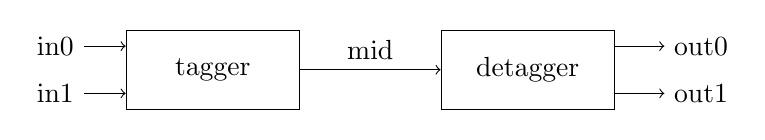
\begin{tikzpicture}
\draw(0,0) node[draw, minimum height = 10mm, minimum width = 22mm] 
  (tagger) {tagger};
\draw(-2,0) node (left){};
\draw ([yshift = 3mm] left) node (in0) {\scalashape in0};
\draw[->] (in0) -- ([yshift = 3mm] tagger.west);
\draw ([yshift = -3mm] left) node (in1) {\scalashape in1};
\draw[->] (in1) -- ([yshift = -3mm] tagger.west);
%
\draw(4,0) node[draw, minimum height = 10mm, minimum width = 22mm]
   (detagger) {detagger};
\draw[->] (tagger) -- node[above] {\scalashape mid} (detagger);
\draw(6.2,0) node (right){};
\draw ([yshift = 3mm] right) node (out0) {\scalashape out0};
\draw[->] ([yshift = 3mm] detagger.east) -- (out0);
\draw ([yshift = -3mm] right) node (out1) {\scalashape out1};
\draw[->] ([yshift = -3mm] detagger.east) -- (out1);
\end{tikzpicture}
\end{center}
%
The intention is that data passed in on |in0| comes out on |out0|; and data
passed in on |in1| comes out on |out1|.  However, there is a single channel
|mid| over which all data has to be passed.  Implement |tagger| and |detagger|
processes, and put them together, to achieve this; use the following
signature. 
%
\begin{scala}
  def multiplex[T](in0: ?[T], in1: ?[T], out0: ![T], out1: ![T]): PROC = ...
\end{scala}

Under what circumstances does your system terminate?  Discuss liveness and
fairness properties of your system.
\end{question}

%%%%%%%%%%%%%%%%%%%%%%%%%%%%%%%%%%%%%%%%%%%%%%%%%%%%%%%

\begin{answer}
Students saw a tagger process like this in lectures.
%
\begin{scala}
  def multiplex[T](in0: ?[T], in1: ?[T], out0: ![T], out1: ![T]): PROC = {
    val mid = OneOne[(Int, T)]

    def tagger = proc{
      serve(
        in0 =?=> { x => mid!(0, x) }
        | in1 =?=> { x => mid!(1, x) }
      )
      in0.close; in1.close; mid.close
    }

    def detagger = proc{
      repeat{
        val (i,x) = mid?(); if(i==0) out0!x else out1!x
      }
      out0.close; out1.close; mid.close
    }
   
    tagger || detagger
  }
\end{scala}

This terminates when either both input channels are closed, or an output
channel for which there is a pending message is closed.  

If the receiver on one of the output channels refuses to take a pending piece
of data, then the system gets stuck, blocking data on the other virtual
channel.  If both receivers are live, then the system is fair to both virtual
channels: if inputs are repeatedly available on both input channels, the
|serve| will alternate between them.
\end{answer}
}
\begin{nontutequestion}
Design a \emph{change machine} process with signature:
%
\begin{scala}
def ChangeMachine(inPound: ?[Unit], out5p: ![Unit], out10p: ![Unit], out20p: ![Unit])
\end{scala}
%
where communications on the channels correspond to the insertion of \pounds 1,
and the output of a 5p, 10p or 20p piece, respectively.  It should be willing
to accept \SCALA{inPound} whenever it had a zero balance.  It should offer
the environment the choice between how it wants the change, subject to the
condition that it should not output coins of more value than it has received. 
\end{nontutequestion}

%%%%%

\begin{nontuteanswer}
\Small
\begin{scala}  
def ChangeMachine(inPound: ?[Unit], out5p: ![Unit], out10p: ![Unit], out20p: ![Unit]) = proc{
  var credit = 0 // credit in pence
  serve(
    (credit == 0 && inPound) =?=> { () => credit += 100 }
    | (credit >= 5 && out5p) =!=> { credit -= 5; () }
    | (credit >= 10 && out10p) =!=> { credit -= 10; () }
    | (credit >= 20 && out20p) =!=> { credit -= 20; () }
  )
}
\end{scala}
\end{nontuteanswer}

%\begin{question}
The CSO construct \SCALA{alt} is rather like the external choice operator
$\extchoice$.  Describe a couple of ways in which they are different.
\end{question}

%%%%%

\begin{answer}
\begin{itemize}
\item
\SCALA{alt} operates over channels, whereas $\extchoice$ operates over
arbitrary processes.  For example, in CSP you can have a process such as
\[
(P \parallel Q) \extchoice (R \intchoice S)
\]
but you can't achieve a similar effect using \SCALA{alt}. 

\item
In CSO, if the outport of a channel is involved in an \SCALA{alt}, the inport
may not simultaneously be involved in an(other) \SCALA{alt}.  But in CSP it's
fine to have a process such as
\[
(c!x \then \ldots \extchoice \ldots) \parallel (c?x \then \ldots \extchoice
\ldots). 
\]
\end{itemize}
\end{answer}

%\begin{nontutequestion}
Recall the following restriction on the use of \SCALA{alt}:
%
\begin{quote}
If the output port of a channel participates in an \SCALA{alt} then its input
end must not simultaneously participate in an(other) \SCALA{alt}.
\end{quote}
%
Suggest a reason for this restriction.
\end{nontutequestion}

%%%%%

\begin{nontuteanswer}
The restriction makes implementation of \SCALA{alt} much easier.  Consider a
program such as \SCALA{P || Q} where:
%
\begin{scala}
def P = proc{ alt( c -!-> ... | a -?-> ...) }
def Q = proc{ alt( c -?-> ... | b -?-> ...) }
\end{scala}
%
The two \SCALA{alt}s are executed by different threads.  There is a danger of
the \SCALA{alt} in \SCALA{P} selecting channel~\SCALA{c} at the same time that
the \SCALA{alt} in \SCALA{Q} selects channel~\SCALA{b}, for example; the two
threads would then evolve in ways inconsistent with the intended semantics.    

Solving these problems would require some non-trivial synchronisation between
the two threads.

This problem potentially becomes harder when we have more than two processes.

Very similar examples can be used to show why the input port of a OneMany
channel may not simultaneously participate in more than one \SCALA{alt}. 
\end{nontuteanswer}

%% Consider a ring of processes:
%% %
%% \begin{scala}
%% || ( for(i <- 0 until N) yield P(i) )
%% \end{scala}
%% %
%% where
%% %
%% \begin{scala}
%% def P(me) = proc{ alt( c((me+1)\%N) -!-> ... | c(me) -?-> ...) }
%% \end{scala}

\begin{question}
% \Programming\
Implement an unbounded buffer as a process:
%
\begin{scala}
def buff[T](in: ?[T], out: ![T]) = proc{ ... }
\end{scala}
%
The process should always be willing to input on \SCALA{in}; it should output
data on \SCALA{out} in the order in which they were received, and should be
willing to output whenever it has input data that have not yet been output. 

{\bf Hint:} you might want to use an instance of a
\SCALA{scala.collection.mutable.Queue} to store the current values held in the
buffer.
\end{question}

%%%%%

\begin{answer}
\Small
\begin{scala}
  def buff[T](in: ?[T], out: ![T]) = proc{
    var queue = new scala.collection.mutable.Queue[T]

    serve(
      in =?=> { x => queue.enqueue(x) }
      | (queue.nonEmpty && out) =!=> { queue.dequeue }
    )
  }
\end{scala}
%
We will discuss testing of datatypes like this later in the course.  For the
moment, I would expect to see some testing involving some threads passing in
pre-defined sequences of values, and other threads taking the outputs and
writing them into global variables, and then checking that the outputs are a
permutation of the inputs. 
%
%% The testing harness is designed to allow data to accumulate in the buffer ---
%% and that's what the test results show.
\end{answer}
%% \begin{answer}
%% \begin{scala}
%% import ox.CSO._

%% object UnboundedBuff{
%%   // Unbounded buffer
%%   def Buff[T](in: ?[T], out: ![T]) = proc{
%%     var queue = new scala.collection.mutable.Queue[T];

%%     serve(
%%       in -?-> { queue.enqueue(in?); }
%%       | (!queue.isEmpty &&& out) -!-> { out!(queue.dequeue); }
%%     )
%%   }

%%   // Produce stream of nats
%%   def Nats(out: ![Int]) = proc("nats"){
%%     var n = 0;
%%     repeat{ out!n; println("Sent "+n); n+=1; sleep(400) }
%%   }

%%   // Consume and print numbers at random intervals
%%   def Console(in: ?[Int]) = proc{
%%     val random = new scala.util.Random;
%%     repeat{ sleep(random.nextInt(1000)); println(in?); }
%%   }

%%   val in, out = OneOne[Int];
%%   def System = Nats(in) || Buff(in, out) || Console(out)

%%   def main(args : Array[String]) = System()
%% }
%% \end{scala}
%% %
%% The testing harness is designed to allow data to accumulate in the buffer ---
%% and that's what the test results show.
%% \end{answer}

\begin{question}
\def\integral#1#2{\int_{#1}^{#2} f(x)\,\mbox{d}x} 
%
\Programming\ Recall the trapezium rule, used for estimating integrals,
discussed in the third chapter.  \emph{Adaptive quadrature} is an
alternative approach that proceeds as follows.  In order to calculate
$\integral{a}{b}$, first compute the midpoint $mid = (a+b)/2$.  Then estimate
three integrals, $\integral{a}{mid}$, $\integral{mid}{b}$ and
$\integral{a}{b}$, each using the trapezium rule with a single interval.  If
the sum of the former two estimates is within some value $\epsilon$ of the
third, then we take that third estimate as being the result.  Otherwise,
recursively estimate the integrals over the two ranges $a$ to~$mid$ and $mid$
to~$b$, and sum the results.  The following sequential algorithm captures this
idea:
%
\begin{scala}
  /** Estimate the integral of f from a to b using adaptive quadrature. */
  def estimate(f: Double => Double, a: Double, b: Double) : Double = {
    val mid = (a+b)/2.0
    val fa = f(a); val fb = f(b); val fmid = f(mid)
    val lArea = (fa+fmid)*(mid-a)/2; val rArea = (fmid+fb)*(b-mid)/2
    val area = (fa+fb)*(b-a)/2
    if (Math.abs(lArea+rArea-area) < Epsilon) area
    else estimate(f,a,mid) + estimate(f,mid,b)
  }
\end{scala}

Write a concurrent program to implement adaptive quadrature.  Give your
program the following signature:
\begin{scala}
class Adaptive(f: Double => Double, a: Double, b: Double, Epsilon: Double, nWorkers: Int){
  require(a <= b)

  def apply(): Double = ...
}
\end{scala}
%
The program should use a bag of tasks with replacement: the two recursive
calls in the sequential version can be implemented by returning tasks to the
bag.  The bag of tasks needs to store the tasks still to be performed: use
either a |Queue| or a |Stack| for this.  You will have to think carefully
about when the system should terminate.

A test harness for this program is on the course website (making use of the
class |TrapeziumTest| from lectures).  Use this to test your code. 
%%%%% /users/gavinl/Teaching/CP/Scala/Trapezium.AdaptiveTest.scala

Suggest ways in which your program can be made more efficient; optional:
implement them.
\end{question}

%%%%%

\begin{answer}
%% We will build a system as illustrated below.
%% %
%% \begin{center}
%% \begin{tikzpicture}
%% \draw(0,0) node[draw] (bag) {\scalashape bag};
%% \draw (3,0) node[draw] (worker) {\scalashape workers};
%% \draw 
%% %% \draw (worker.north east)++(0.2,0.2) node (control1) {};
%% %% \draw (worker.south east)++(0.2,0.2) node (control2) {};
%% %% \draw (worker.north west)++(0.2,0) -- ++ (0,0.2) -- (control1) --
%% %% (worker.south east)++(0.2,0.2); %(control2);
%% \end{tikzpicture}
%% \end{center}
My code is below.  To support termination, the bag keeps track of the
number of workers currently working on a task; a worker informs the
bag that it has completed a task via the channel |done|.  When the bag
is empty and there are no busy workers, the bag closes the channels to
terminate the system.
%
\begin{scala}
/** Calculating integral, using trapezium rule, adaptive quadrature, and bag
  * of tasks pattern. */
class Adaptive(f: Double => Double, a: Double, b: Double, Epsilon: Double, nWorkers: Int){
  require(a <= b)

  /** A task is an interval on which to work. */
  private type Task = (Double, Double)

  /** Channel from the controller to the workers, to distribute tasks.  We
    * create the channel freshly for each run of the system. */
  private val toWorkers = OneMany[Task] 

  /** Channel from the workers to the bag, to return subtasks. */
  private val toBag = ManyOne[(Task,Task)]

  /** Channel from the workers to the adder process, to add up subresults. */
  private val toAdder = ManyOne[Double]

  /** Channel to indicate to the bag that a worker has completed a task. */
  private val done = ManyOne[Unit]

  /** A client, who receives arguments from the server, either estimates the
    * integral directly or returns new tasks to the bag. */
  private def worker = proc("worker"){
    repeat{
      val (a,b) = toWorkers?()
      val mid = (a+b)/2.0
      val fa = f(a); val fb = f(b); val fmid = f(mid)
      val lArea = (fa+fmid)*(mid-a)/2; val rArea = (fmid+fb)*(b-mid)/2
      val area = (fa+fb)*(b-a)/2
      if (Math.abs(lArea+rArea-area) < Epsilon) toAdder!area
      else toBag!((a,mid), (mid,b)) 
      done!(())
    }
  }

  /** The bag, that keeps track of jobs pending. */
  private def bag = proc("bag"){
    val stack = new scala.collection.mutable.Stack[Task]
    stack.push((a,b))
    var busyWorkers = 0 // # workers with tasks

    serve(
      (stack.nonEmpty && toWorkers) =!=> { busyWorkers += 1; stack.pop }
      | (busyWorkers > 0 && toBag) =?=> { case (t1,t2) =>
          stack.push(t1); stack.push(t2) }
      | (busyWorkers > 0 && done) =?=> { _ => busyWorkers -= 1 }
    )
    // busyWorkers == 0 && stack.isEmpty
    toWorkers.close; toAdder.close
  }

  private var result = 0.0

  // Process to receive results from workers and add up the results
  private def adder = proc("adder"){ repeat{ result += (toAdder?()) } }

  def apply(): Double = {
    val workers = || (for (i <- 0 until nWorkers) yield worker)
    run(workers || bag || adder)
    result
  }
}
\end{scala}

%% Testing can be done in a very similar way to as in lectures, by testing
%% against a sequential implementation.  The main part of my code is below.  The
%% function |pickParams| picks parameters.  The function |estimate| is as in the
%% question.
%% %
%% \begin{scala}
%%   /** Do a single test. */
%%   def doTest = {
%%     val (f, p, a, b, nWorkers) = pickParams
%%     val seqResult = estimate(f, a, b)
%%     val concResult = new Adaptive(f, a, b, Epsilon, nWorkers)()
%%     assert(
%%       seqResult != 0.0 && Math.abs((seqResult-concResult)/seqResult) < 1E-7 ||
%%         Math.abs(seqResult-concResult) < 1E-10, ...)
%%   }
%% \end{scala}

Here are four ways this could be made more efficient.  Each aims to reduce
the number of communications (since communications are expensive).
%
\begin{itemize}
\item
Above the worker returns two tasks to the bag, and then (on the next
iteration) gets one back, possibly one of the tasks it just put there.  It
would be more efficient to just return one and to continue calculating with
the other.  In particular, the bag is likely to be a bottleneck, and this
reduces the load on the bag.

\item
The trapezium rule is applied to most intervals twice: once before that
interval is placed in the bag, and once when it is retrieved.  It would be
more efficient to put the calculated estimate into the bag along with the
interval, so it doesn't need to be recalculated.

\item
We could arrange for a |done| message to be sent only when the worker
does not return subtasks to the bag: the bag can infer that the worker
is done in the other case.

\item 
Each worker could accumulate sub-results in a thread-local variable, and send
to the adder only at the end. 

% \item
% We could merge the \SCALA{Adder} with the \SCALA{Bag}, and do away with the
% \SCALA{done} events.  All the workers will be idle if the number of tasks
% distributed equals the number of results received, plus half the number of
% tasks returned to the bag.  (If the change in the first bullet point is
% implemented, then that condition becomes that the number of tasks
% distributed equals the number of results received.)
\end{itemize}
\end{answer}


%\begin{nontutequestion}
\Programming\
Recall the integrator network from the previous sheet.  Adapt the network so
that it has an additional input channel 
\SCALA{reset : ?[Unit]}, such that when it receives a signal on
\SCALA{reset}, the current sum gets reset to 0.  Explain your design.  {\bf
  Hint:} you only need to change one component of the network.
\end{nontutequestion}

%%%%%

\begin{nontuteanswer}
\Small
We replace the \SCALA{prefix(0)} component with a new component
\SCALA{Control} which handles the resets:
%
\begin{verbatim}
                in                       out
 [x,y,z,...] >------>|\    mid     /|-------> [x,x+y,x+y+z,...]
                     |+}--------->{ |
                 +-->|/            \|--+
             addl|                     |back
                 +------<Control<------+
                           /|\
                            |
                          reset
\end{verbatim}
%
It's also possible to put the resetting component elsewhere in the network.

Note that \SCALA{Control} needs to absorb the sum currently circulating before
(or after) injecting a fresh value~$0$.  It makes sense to give \SCALA{reset}
priority over values currently circulating.
%
\begin{scala}
import ox.CSO._, ox.cso.Components

object ResettableIntegrator{

  def Control(in: ?[Int], out: ![Int], reset: ?[Unit]) 
  = proc{
    out!0;
    priserve(
      reset --> { 
        reset?; println("Resetting"); in?; out!0 
      }
      | in --> { out!(in?) }
    )
  }  

  def integrator(in: ?[Int], out: ![Int], reset: ?[Unit])
  = {
    val mid, back, addl = OneOne[Int]
    (Components.zipwith((x:Int, y:Int)=>x+y)(in, addl, mid)
    || Components.tee (mid, List(out, back))
    || Control(back, addl, reset)
    )
  }

  // Produce stream of nats
  def Nats(out: ![Int]) = proc("nats"){
    var n = 0;
    repeat{ out!n; n+=1; sleep(200) }
  }

  // Randomly reset
  def Resetter(reset: ![Unit]) = proc{
    val random = new scala.util.Random;
    repeat{ sleep(random.nextInt(1000)); reset!(); }
  }  

  // Test rig, using the above
  def TestRig = {
    val in, out = OneOne[Int]; val reset = OneOne[Unit];
    ( integrator(in, out, reset) || 
     Nats(in) || Resetter(reset) || 
     Components.console(out) )
  }

  def main(args : Array[String]) = TestRig()
}
\end{scala}

\end{nontuteanswer}

%\begin{nontutequestion}
\Programming\ 
The \emph{readers and writers problem} is a classic synchronisation problem.
Consider a collection of processes, each of which want to access a database
concurrently, some for reading and some for writing.  It is allowable for
several readers to be accessing the database simultaneously, since their
transactions will be independent.  However, it is not allowable for two
writers to have simultaneous access, nor for a reader and writer to have
simultaneous access.

Implement a solution to the readers and writers problem using a server
process: each reader and writer should communicate with the server when
entering or leaving.

Is a reader or writer who is trying to gain entry to the database guaranteed
to succeed, or could it be locked out forever?  If the latter, how could this
be avoided? 
\end{nontutequestion}

%%%%%

\begin{nontuteanswer}
\Small
The server needs to keep track of the numbers of readers and writers currently
accessing the database, and maintain the invariant
\[
(readers=0 \land writers \le 1) \lor writers=0
\]

Avoiding starvation is tricky, since, say readers may always gain access,
locking the writers out for ever.  Below, priority is given to processes
wishing to leave, and when $readers=0 \land writers=0$, it alternates between
giving priority to a reader or a writer (according to the flag
\SCALA{writerPri}).    
%
\begin{scala}[showstringspaces=false]
// The readers and writers problem
import ox.CSO._

object ReadersWriters{
  val random = new scala.util.Random;

  // A reader, which just repeatedly enters and leaves
  def Reader(me: Int, enter: ![Int], leave: ![Int]) = proc{
    repeat{
      sleep(random.nextInt(2000)); enter!me;
      sleep(random.nextInt(1000)); leave!me
    }
  }

  // A reader, which does likewise
  def Writer(me: Int, enter: ![Int], leave: ![Int])= proc{
    repeat{
      sleep(random.nextInt(2000)); enter!me;
      sleep(random.nextInt(1000)); leave!me
    }
  }

  // A server which controls the entering and leaving, 
  // maintaining the invariant: (readers==0 && writers<=1) || writers==0
  // Priority is always given to leaving.  When readers==0 and writers==0, 
  // priority is given to a writer to enter next iff writerPri
  def Server(readerEnter: ?[Int], readerLeave: ?[Int],
	     writerEnter: ?[Int], writerLeave: ?[Int])
  = proc{
    var readers = 0; var writers = 0;
    def Report = { println("readers="+readers+"; writers="+writers); }
    var writerPri = true; // Does writer get priority?

    priserve(
      (readers>0 &&& readerLeave) --> {
	val id = readerLeave?; readers-=1; println("Reader "+id+" leaves"); Report
      }
      | 
      (writers>0 &&& writerLeave) --> {
	val id = writerLeave?; writers-=1; println("Writer "+id+" leaves"); Report
      }
      | 
      (writerPri && readers==0 && writers==0 &&& writerEnter) --> {
	val id = writerEnter?; writers+=1; writerPri=false;
	println("Writer "+id+" enters"); Report
      }
      |
      (writers==0 &&& readerEnter) --> {
	val id = readerEnter?; readers+=1; writerPri=true;
	println("Reader "+id+" enters"); Report
      }
      | 
      (!writerPri && readers==0 && writers==0 &&& writerEnter) --> {
	val id = writerEnter?; writers+=1; writerPri=false;
	println("Writer "+id+" enters"); Report
      }
    )
  }

  // Number of readers and writers:
  val readers = 5; val writers = 5

  // Declare the channels
  val readerEnter, readerLeave, writerEnter, writerLeave = ManyOne[Int];  

  def Readers = 
    || ( for(i <- 0 until readers) yield Reader(i, readerEnter, readerLeave) )
  def Writers =
    || ( for(i <- 0 until readers) yield Writer(i, writerEnter, writerLeave) )
  def System = 
    Readers || Writers || Server(readerEnter,readerLeave,writerEnter,writerLeave)

  def main(args : Array[String]) = { System() }
}
\end{scala}

This does not guarantee starvation freedom, since the readers may try to enter
sufficiently often that $readers$ never reaches zero, so no writer can gain
entry.  This can be avoided by having writers register their interest (by
another communication, that the server always accepts), and then not allowing
any more \SCALA{readerEnter} events before a \SCALA{writerEnter} event.
\end{nontuteanswer}


%% Loosely based on A7.9
\begin{question}
\Programming\ Consider a setting with two kinds of processes, which we will
call Male and Female; suppose we have $N$ Males and $N$ Females.  The aim is
to pair the processes off for some purpose, so each Male is paired with a
Female, and vice versa.  Each process should end up in possession of its
partner's identity.  Design and implement a protocol to achieve this.  The
protocol should be such that the pairings are decided nondeterministically (so
it's not acceptable for the protocol to simply pair each Male off with the
Female with the same index, for example).  The protocol should not use any
process other than the Males and Females.  Note: you need to be careful to
follow the restrictions on the use of \SCALA{alt}s.
\end{question}

%%%%%

\begin{answer}
We will arrange (arbitrarily) for the Female to send a ``proposition'' to a
Male, and she is willing for any Male to receive this; each Male will accept a
single proposition, and is willing to accept it from any Female.  (I'm not
sure which gender this is less polite towards!)   

It is worth considering the type of the proposition channel.  One approach
that doesn't work is to have $N^2$ \SCALA{OneOne} channels, so that Female~$i$
propositions Male~$j$ on channel \SCALA{prop(i)(j)}; this would mean that
Female~$i$ would use an \SCALA{alt} over the output ports of the
\SCALA{prop(i)(j)}, for $j = 0, \ldots, N-1$; and that Male~$j$ uses an
\SCALA{alt} over the input ports of the \SCALA{prop(i)(j)}, for $i = 0,
\ldots, N-1$; but that breaks one of the restrictions on the use of
\SCALA{alt}.

Another approach that doesn't work is to give each Female a \SCALA{OneMany}
proposition channel, on which it can send a proposition to an arbitrary Male.
However, then each Male would use an \SCALA{alt} over the input ports of those
channels, breaking the other restriction on the use of\SCALA{alt}.

The approach we do take is to use a single \SCALA{ManyMany}
channel~\SCALA{prop}, on which an arbitrary Female may proposition an
arbitrary Male.  The Female can send her identity within the proposition.  The
Male can then respond, sending his own identity; we give each Female a
\SCALA{ManyOne} channel for this.
%
\begin{scala}
import ox.CSO._

object MaleFemale{
  val N = 5; // number of males and females

  def Female(me: Int, prop: ![Int], resp: ?[Int]) 
  = proc("Female "+me){
    prop!me;
    val him = resp?;
    report!("Female "+me+" coupled with male "+him);
  }

  def Male(me: Int, prop: ?[Int], resp: Seq[![Int]]) 
  = proc("Male "+me){
    val her = prop?;
    resp(her)!me;
    report!("Male "+me+" coupled with female "+her);
  }

  val prop = ManyMany[Int];
  val resps = ManyOne[Int](N);
  val report = ManyOne[String]

  val System = (
    || ( for(i <- 0 until N) 
           yield Female(i, prop, resps(i)) )
    || 
    || ( for (i <- 0 until N) 
           yield Male(i, prop, resps) )
    || ox.cso.Components.console(report) 
  );

  def main(args : Array[String]) = System();
}
\end{scala}
\end{answer}

    


%%%%% clients & servers

\input{menWomenServer}

%%%%% interacting peers
\input{ringFold}
\begin{question}
Consider a system constructed from $N$ similar processes, with identities
$0, \ldots, N-1$.  Each process can send messages to any other process, on
synchronous channels.

Each process is either \emph{active} or \emph{passive}.  When a process is
passive, it simply waits to receive a message, at which point it becomes
active.  When a process is active, it can send messages to any other
processes, but may eventually become passive.

The aim of this question is to consider a technique for determining whether
all the processes are passive, in which case the system can terminate.

\begin{enumerate}
\item Consider the following scheme.  Process~0, when it is passive, sends a
token to process~1, containing a boolean value, initially $true$.  Each
process~$k$, when it receives a token of this form, sends a similar token to
process~$(k+1) \bmod N$, so the token circulates, as if the processes are
arranged in a ring; note, though that other messages don't need to follow the
ring.  Process~$k$ sets the value in the token to be $false$ if it is active,
or passes on the value it receives if it is passive; in each case, the process
retains its previous status (active or passive).  When the token returns to
process~0, if its value is $true$, it assumes that all processes are passive,
so sends a message to all processes telling them to terminate.

Explain why this scheme does \emph{not} achieve the desired goal.

%%%%%

\item
Describe how to adapt this scheme so that it does achieve the desired goal.
Explain why your scheme works.  Make clear what (safety and liveness)
properties your scheme achieves.

%%%%%

\item
Now suppose the normal messages do follow the ring topology.  Describe how to
adapt the scheme so that it achieves the desired goal. 

% \item
% Does it make a difference if the channels are asynchronous (i.e.~buffered)? 
\end{enumerate}
\end{question}

%%%%%%%%%%%%%%%%%%%%%%%%%%%%%%%%%%%%%%%%%%%%%%%%%%%%%%%

\begin{answer}
\begin{enumerate}
\item
Consider a ring of four processes, with process~3 initially active.  Suppose
the token circulates to process~2, so the boolean is still $true$.  Then
suppose process~3 sends a message to process~1 and becomes passive, but
process~1 remains active.  Then the token is passed on to process~3, then
back to process~0, with the boolean still $true$.  Hence process~0 assumes all
processes are passive, even though process~1 is active.

%%%%%

\item Arrange for the token to go round the ring \emph{twice} (with some field
indicating whether it is on its first or second circuit).  On the second
circuit, each process sets the boolean to be $false$ if it has been active at
any time since it saw the token the first time.

Consider the time~$t$ at which the token first returns to process~0.  If
any process is active at time~$t$, then it will subsequently set the boolean
to $false$.  Hence, if the value ends up $true$, then all processes were
passive at time~$t$, and so all remain passive.  (This is a safety property:
the system terminates only if it is correct to do so.) 

It is possible for all the processes to become passive while the token is
circulating, but after at least one has seen it for the first time, in which
case the scheme does not lead to overall termination.  However, if all are
passive when the token starts circulating for the first time, then termination
will result.  (This is a liveness property: the system does terminate,
under the stated conditions.)


%%%%%

\item Arrange for the termination messages and the data messages to go round
the ring in the same direction.  Sending the token only once round the ring is
now sufficient: process~0 can choose to terminate provided the boolean comes
back as $true$ and it has been continually passive since initiating the token.
The following property is invariant: if process~0 remains passive, and the
boolean in the token is still $true$, then all processes between~0 and the
current token-holder are passive.

\emph{Alternatively} send the termination messages round the ring in the
\emph{opposite} direction, i.e.~node~$i$ sends the termination token to
node~$(i-1) \bmod N$.   The following property is invariant: if process~$i$
sends the token with value $true$, then all processes in the range $[i ..
N-1) \union \set{0}$ are passive.


% \item
% If the channels are asynchronous, then each passive process must check that
% its input channels are empty before passing the token.  Otherwise, such a
% process could subsequently become active as a result of receiving a message
% that was in the channel.

\end{enumerate}
\end{answer}
 % Distributed termination
\end{document}
